
\begin{figure}[H]
\minipage{0.49\textwidth}
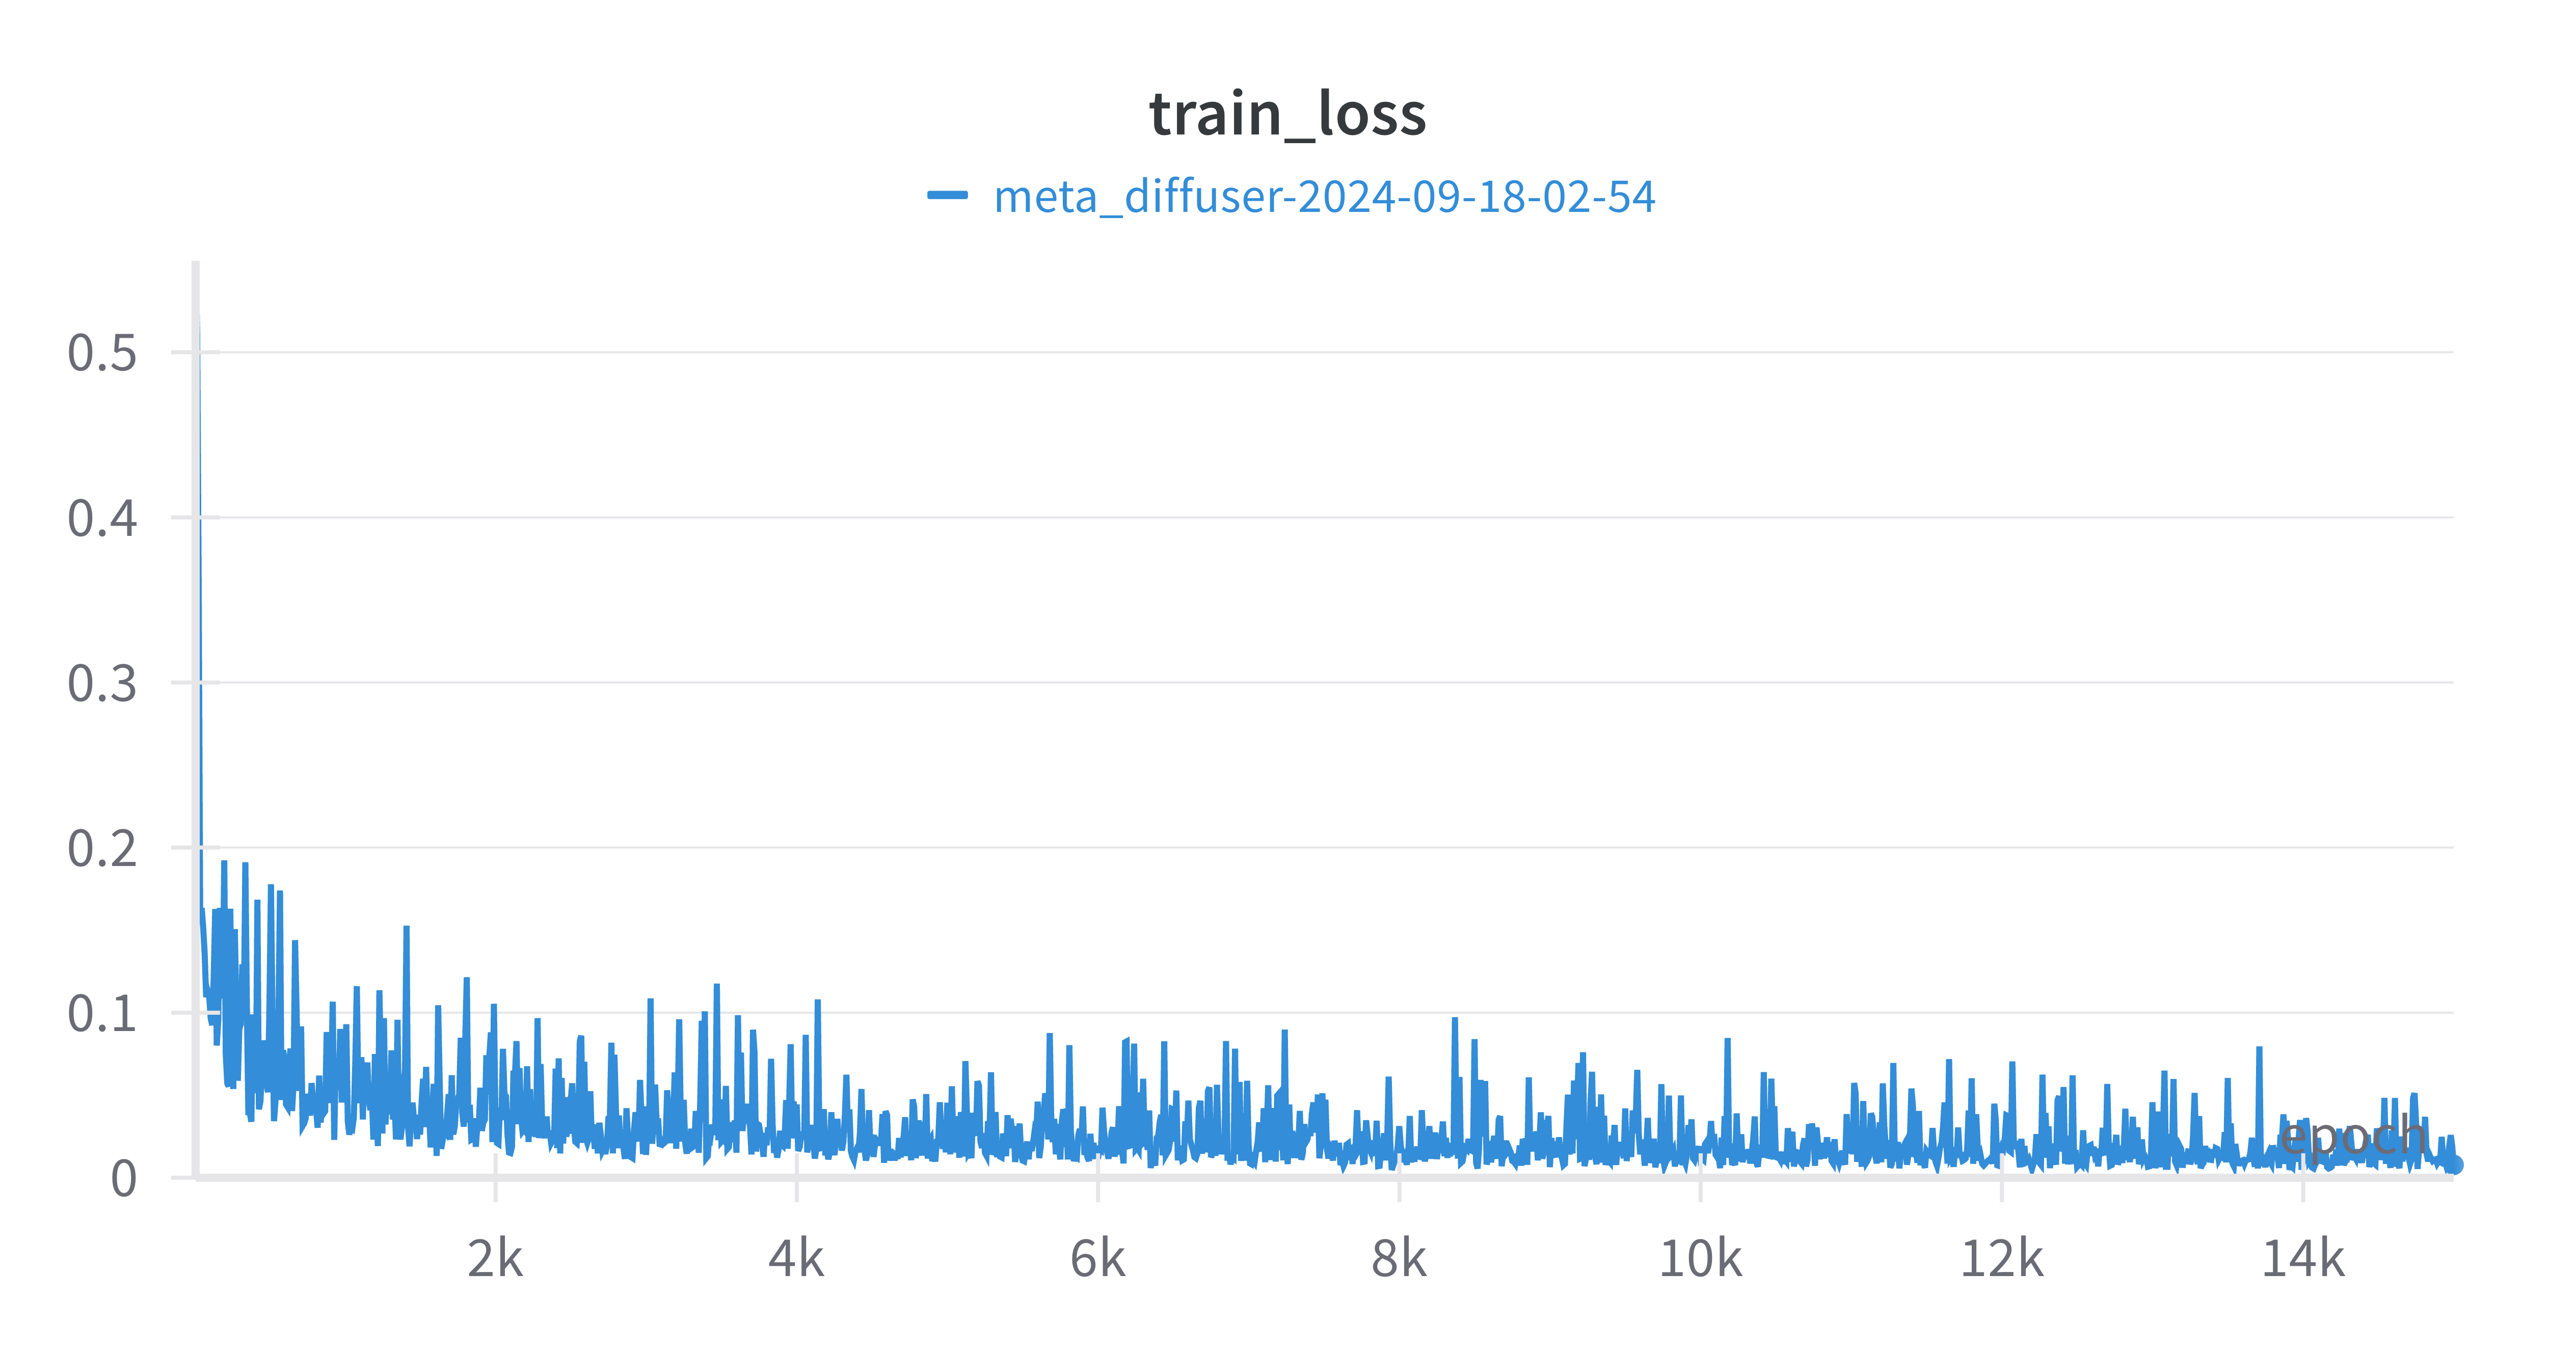
\includegraphics[width=\linewidth]{detailed_engineering/Meta Diffusion/charts/train_loss.png}
\caption{Loss during the training. Lower is better.}
\endminipage\hfill
\minipage{0.49\textwidth}
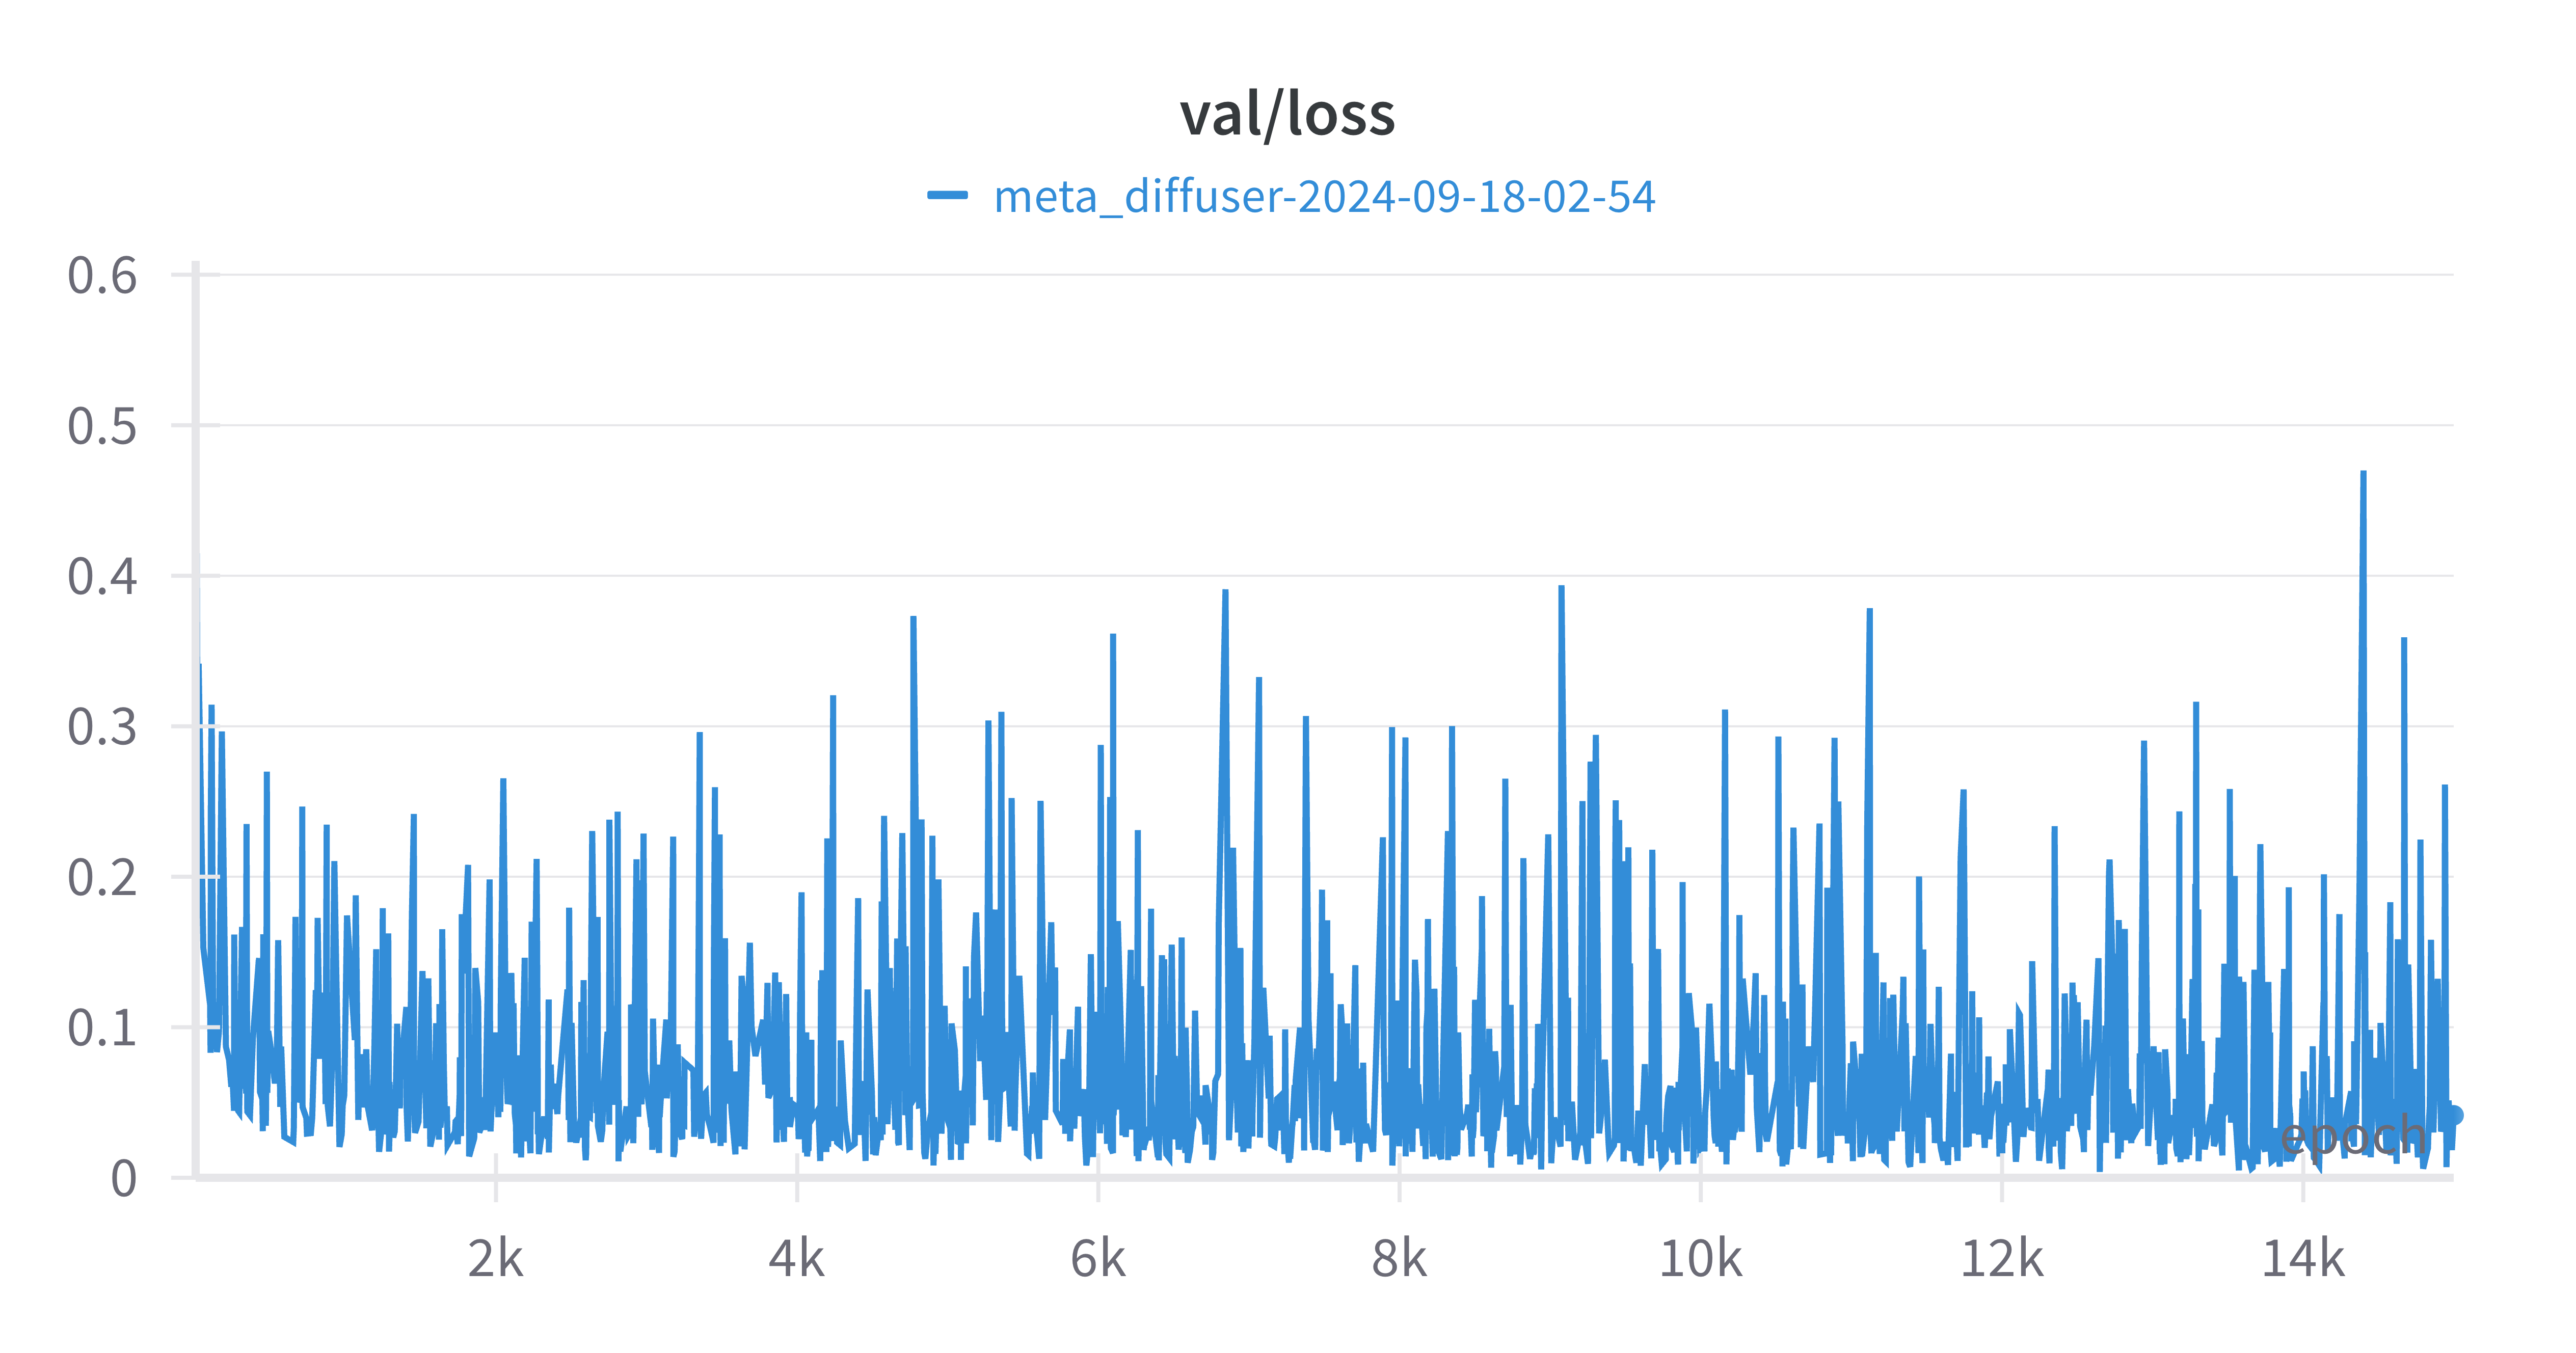
\includegraphics[width=\linewidth]{detailed_engineering/Meta Diffusion/charts/val_loss.png}
\caption{Loss during the validation. Lower is better.}
\endminipage
\end{figure}

Additional metrics evaluating the quality of the generated scan.
\begin{figure}[H]
\minipage{0.49\textwidth}
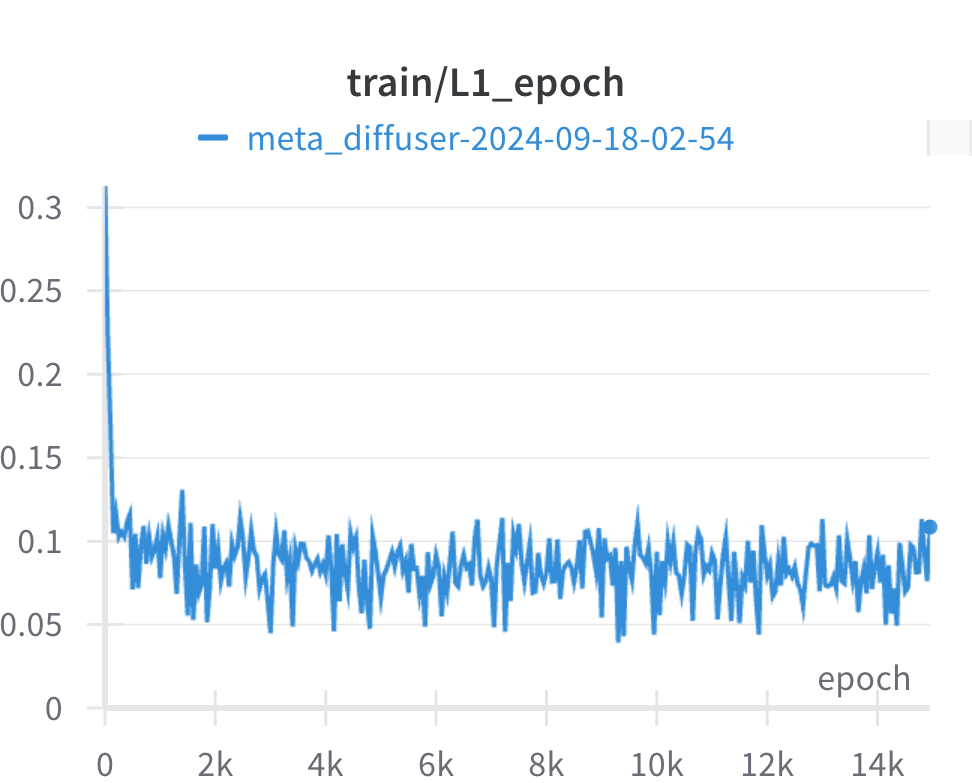
\includegraphics[width=\linewidth]{detailed_engineering/Meta Diffusion/charts/train_l1_epoch.png}

\endminipage\hfill
\minipage{0.49\textwidth}
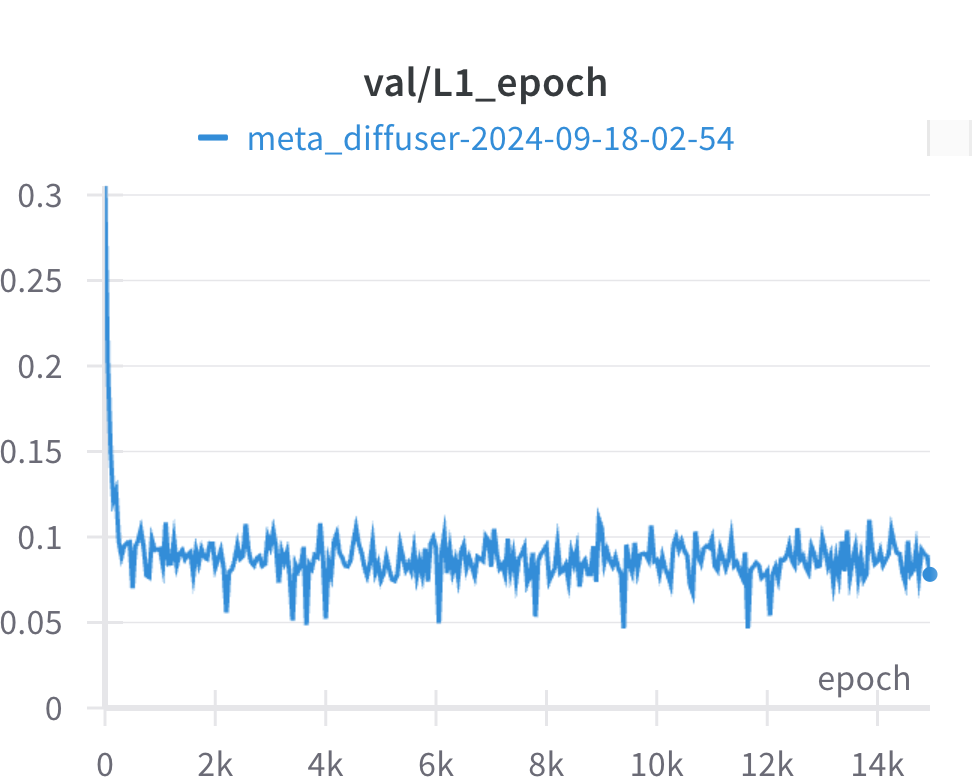
\includegraphics[width=\linewidth]{detailed_engineering/Meta Diffusion/charts/val_l1_epoch.png}

\endminipage
\caption{L1 between two generated CT scans and two random samples from training/validation datasets. Lower is better.}
\end{figure}

\begin{figure}[H]
\minipage{0.49\textwidth}
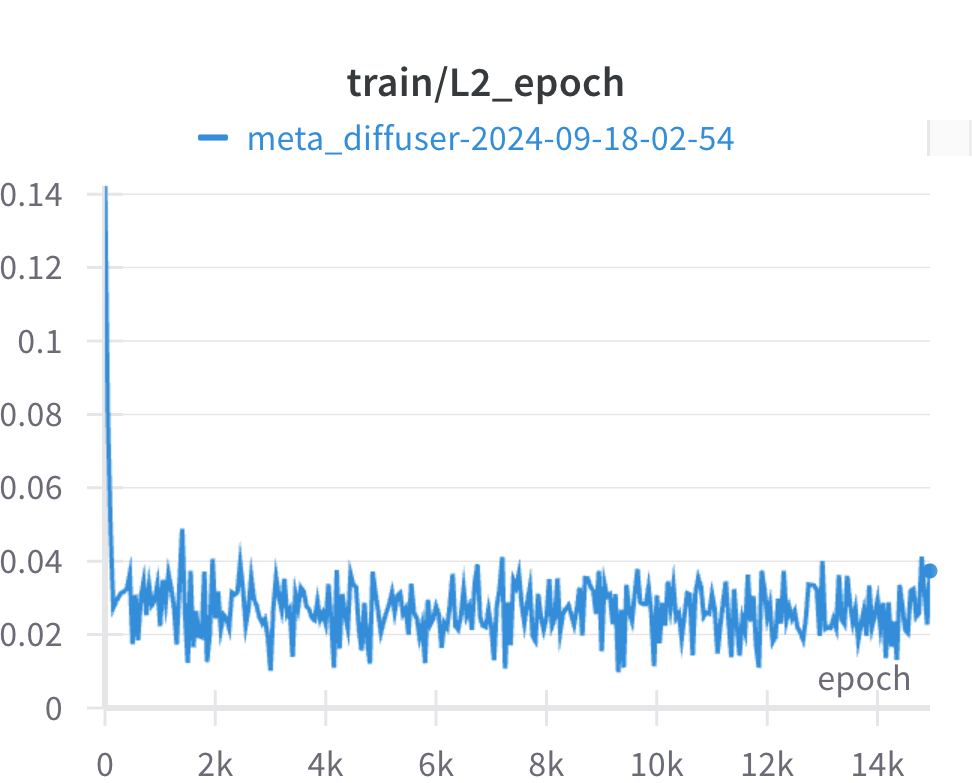
\includegraphics[width=\linewidth]{detailed_engineering/Meta Diffusion/charts/train_l2_epoch.png}

\endminipage\hfill
\minipage{0.49\textwidth}
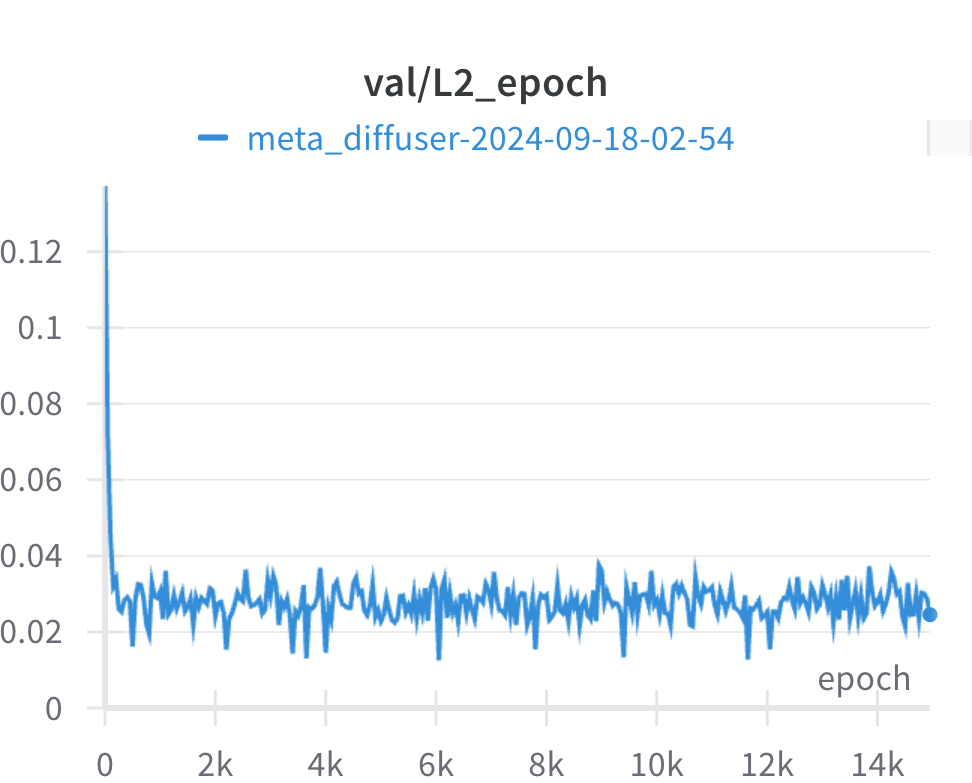
\includegraphics[width=\linewidth]{detailed_engineering/Meta Diffusion/charts/val_l2_epoch.png}

\endminipage
\caption{L2 between two generated CT scasn and two random samples from training/validation datasets. Lower is better.}
\end{figure}

\begin{figure}[H]
\minipage{0.49\textwidth}
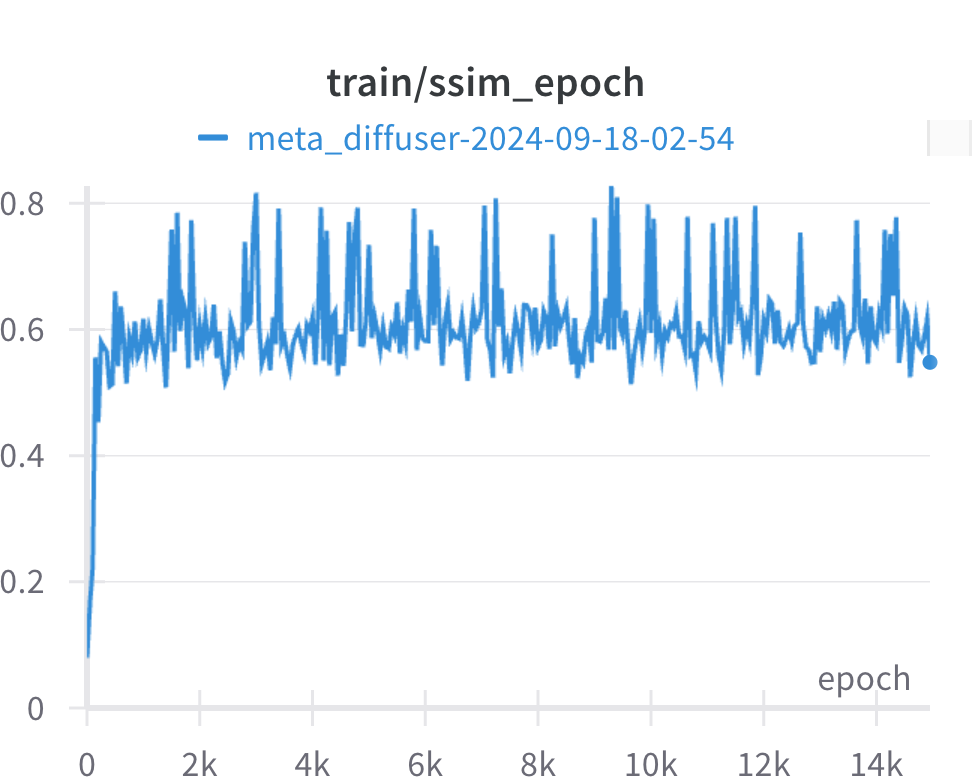
\includegraphics[width=\linewidth]{detailed_engineering/Meta Diffusion/charts/train_ssim_epoch.png}

\endminipage\hfill
\minipage{0.49\textwidth}
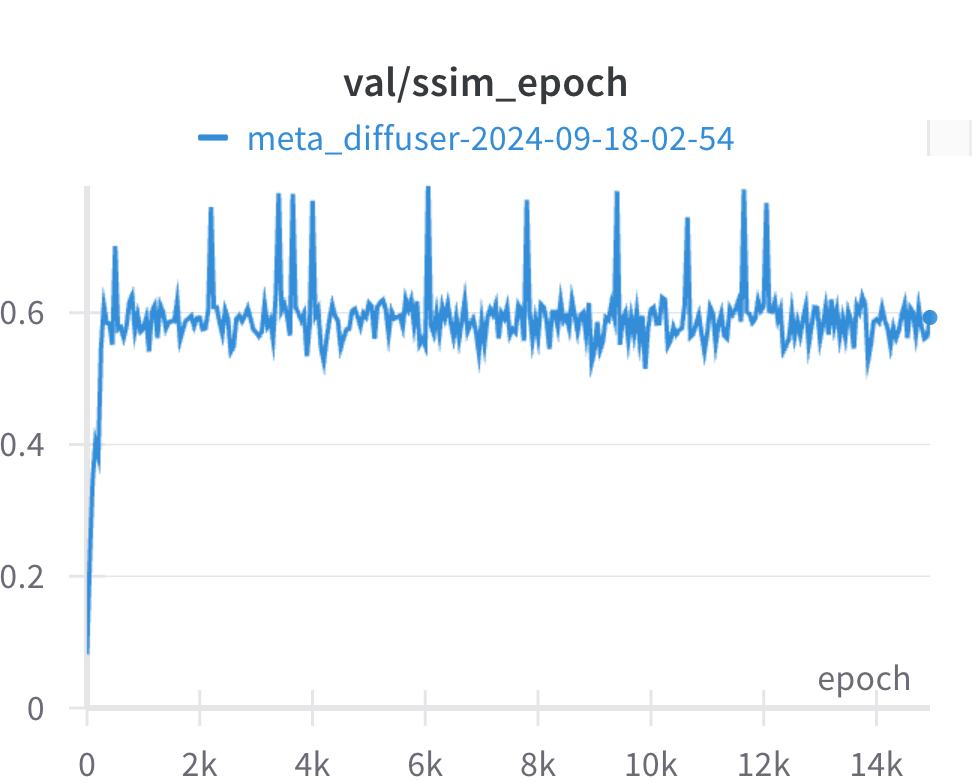
\includegraphics[width=\linewidth]{detailed_engineering/Meta Diffusion/charts/val_ssim_epoch.png}

\endminipage
\caption{MSSIM between two generated Ct scans and two random samples from training/validation datasets. Higher is better.}
\end{figure}

\paragraph{Results}\mbox{}\\

% \begin{figure}[H]
%     \centering
%     \includegraphics[width=\linewidth]{}
%     \caption{Caption}
%     \label{fig:enter-label}
% \end{figure}
\begin{figure}[H]
    \centering
    % \includegraphics{}
     \animategraphics[width=\textwidth, loop, autoplay]{5}%frame rate
    {detailed_engineering/Meta Diffusion/generation/layer-}%path to figures
    {0}%start index
    {31}%end index
    \caption{Random layer of synthetic CT scan generated from Gaussian noise.}
    \label{fig:my_label}
\end{figure}

\begin{figure}[H]
    \centering
    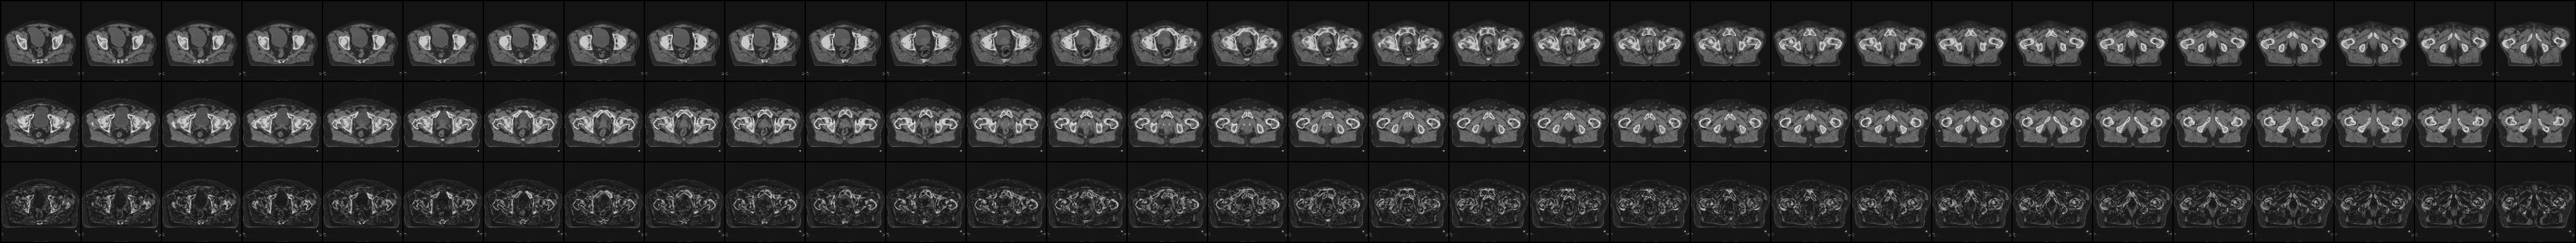
\includegraphics[width=\linewidth]{detailed_engineering/Meta Diffusion/charts/meta_diffusion_comparison.png}
    \caption{Top - first sample from trianing dataset, middle - synthetic CT scan, bottom - L1 difference between them.}
    \label{fig:ldm-success-comparison}
\end{figure}